\section{Early detection of potential failing students}

\label{sec:strategy}

Identifying potential failing students early is very important in the sense that professors still have enough time to act and avoid students to fail the course. In this paper, we focus exclusively on identifying these students. Providing and reporting a technique useful to reduce the failure rate is outside the scope of this paper. Nevertheless, notice that when identifying these students and learning the cause of the failings, we can provide a technique to reduce the aforementioned rate. In fact, based on the results of this paper, we intend to propose a technique to reduce the failure rate as future work.

Next, we detail our strategy to identify these students.

\subsection{Online judge system}
% This section should answer: Why is this kind of system important to identify potential falling students?
% Answer: We need metrics. In order to discover how students are performing, it is necessary a close monitoring of students behaviour
% Talk about Huxley, only enough to explain the metrics: submissions and submission_status (Correct ...)
In order to discover how students are performing, it is important to define a strategy to close monitoring students’ behavior. This strategy should include a way to extract metrics from students. Online learning tools may be a source for these metrics. In the context of programming, a very popular category of systems is the online judges. These systems present students to a set or programming problems. The students solve the problem using a programming language and then submits their solutions. The online judge runs the student’s solution against a set of test cases and in the case the solution passes over all the tests it will be evaluated as correct, otherwise, it will be evaluated according to the type of error, such as wrong answer, compilation error, runtime error, etc.

% Why the Huxley and not others?
% answer: Metrics and performance improvement (not in scope)
In our strategy, we choose to use an online judge named \emph{The Huxley} \cite{paes2013ferramenta} to collect metrics from our students. In this system, the judge provides one of the following outputs for a submission: correct, wrong answer, time limit exceeded, compilation error, runtime error, presentation error and empty answer. We will use these outputs as the main source of metrics. This particular online judge system was chosen because it has some features that we believe will be useful to improve the overall performance of students as a future direction of this research. More specifically, the tool will support us to deal with the following problems:
\begin{itemize}
  \item Students only learn how to program by programming~\cite{jenkins-ltsn02}. The Huxley provides a database composed of more than 300 problems. It allows students to submit their solutions to any of these problems and they are encouraged to try once mistakes are not penalized.
  \item Sometimes a student misses a basic concept and then cannot follow the next lecture. She believes that there is no going back; the course is behaving at a speed that she thinks she will be not able to follow. Such a student will quickly come to the view that ``they just cannot do programming'', and will attribute this to the perceived difficulty of the subject. In other words, students learn at different speeds. As the tool is available online on the Internet, each student can find its own rhythm.
  \item Students need rapid feedback. Many professors are overwhelmed with their daily activities. Then they have no time to give feedback on every student code. On the other side, students need this feedback to continue their learning process in the right path. The Huxley provides a feedback right after a student submits her code. The feedback indicates whether the student's code produces the right answer and gives tips otherwise.
  \item There always be great students and bad students. The great ones should be presented to challenges that make them even greater and the bad ones should be presented to a different set of problems that allow them to become better. Each programming problem of the Huxley is classified according to this level of difficulty and the programming topics it covers. This allows each student to choose the next problem in accordance with this level of expertise.
\end{itemize}

\subsection{Metrics}

\label{sec:metrics}

We use two metrics in our strategy. We explain them in what follows:

\begin{itemize}

	\item \textbf{Number of submissions:} this metric represents the number of submissions a student do during the course. As explained, Huxley provides more than 300 programming exercises. To solve a particular problem, a student needs to submit at least one solution.

	\item \textbf{Number of correct submissions:} if a student solves one problem, we increase this metric by one.

\end{itemize}

Depending on the level of difficulty of a problem, students may submit several times to solve it. However, notice that this is not necessarily a bad thing regarding the learning process. For example, submitting many times means that students are somehow practicing and studying continuously. Thus, although she is not hitting a right solution, she is trying hard and will eventually hit one. Thus, the number of submissions metric is a good indicator of the amount of practice, which is frequently associated with the level of engaging and learning. However, when considered isolated, a high number of submission may also mean that the student is getting frustrated due to so many wrong answers she receives. This way, we also consider the number of correct submissions to compensate and help us on studying such cases as well.

\todo{Referencia do Ig pode ajudar a responder porque as metricas sao boas.}

\subsection{Clustering algorithm}

To identify potential failing students, we use a clustering algorithm to define groups of students. Our idea consists of identifying different groups of students so that we can clearly separate students susceptible to fail from the other ones. To compute the groups, the algorithm takes into account the metrics we present in Section~\ref{sec:metrics}. To make the strategy parameterizable in terms of number of groups, we use the well-known clustering algorithm k-means~\cite{}, which takes such a number as input.

Notice that the number of groups plays an important role on identifying potential failing students. In this paper, we set the algorithm to compute two and three groups and evaluate both cases. When considering two groups, we define them as the students who will either fail or pass. For three groups, we have fail, pass, and students in which the strategy cannot conclude anything about them, which we name ``inconclusive." This is reasonable since our study focuses on the very first 30 days, which means that our drawings regarding the inconclusive group might be completely wrong: these students can either improve themselves and pass the course or fail due to several reasons.

We focus on two and three groups because (i) using one group is useless; and (ii) more than three may lead the strategy to define many groups where it cannot conclude anything. By using three, we have only one group where this happens. \todo{Nao tenho certeza se precisamos explicar isso.}

\subsection{Summary}

Figure~\ref{fig:strategy} combines all steps of our strategy. As the classes are happening, students are encouraged to solve the problems available at Huxley. Although solving exercises is not mandatory, there some particular activities where the professor forces students to use Huxley, such as formal exams. Next, we collect the metrics we detail in Section~\ref{sec:metrics}. To identify potential failing students \textit{early}, we collect the metrics for the first 30 days of the introductory programming courses. Then, we execute the k-means clustering algorithm.

\begin{figure}[htb]
\centering
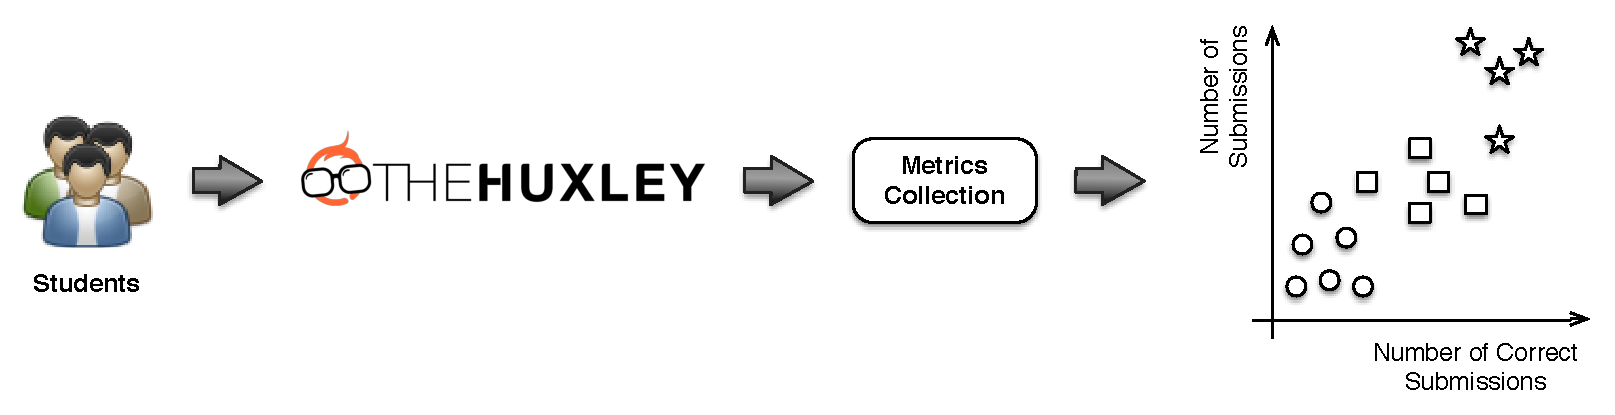
\includegraphics[width=1.0\textwidth,natwidth=610,natheight=642]{images/Strategy.pdf}
\caption{Summary of our strategy to identify potential failing students.}
\label{fig:strategy}
\end{figure}